% Created 2024-09-10 Tue 17:34
% Intended LaTeX compiler: pdflatex
\documentclass[11pt]{article}
\usepackage[utf8]{inputenc}
\usepackage[T1]{fontenc}
\usepackage{graphicx}
\usepackage{longtable}
\usepackage{wrapfig}
\usepackage{rotating}
\usepackage[normalem]{ulem}
\usepackage{amsmath}
\usepackage{amssymb}
\usepackage{capt-of}
\usepackage{hyperref}
\usepackage{minted}
\usepackage{xcolor}
\usepackage{hyperref}
\usepackage{tocloft}
\usepackage[margin=1.8cm]{geometry}
\usepackage{fancyheadings}
\usepackage{minted}
\usepackage[utf8]{inputenc}
\usepackage{amsmath}
\usepackage{amsfonts}
\usepackage{amssymb}
\usepackage{titlesec}
\usemintedstyle{manni}
\usepackage{enumitem}
\usepackage{pdfpages}
\setlength{\parindent}{0cm}
\usepackage{parskip}
\usemintedstyle{friendly}
\usepackage{graphicx}
\usepackage{listings}
\usepackage{float}
\usepackage{colortbl}
\usepackage{booktabs}
\usepackage{wrapfig}
\usepackage{tabularx}
\usepackage{color}
\usepackage{tabularray}
\restylefloat{table}
\usemintedstyle{dracula}
\usepackage[table]{xcolor}
\usepackage{setspace}
\usepackage[none]{hyphenat}
\usepackage{xcolor}
\usepackage{pagecolor}
\definecolor{solarizedBase03}{RGB}{0, 43, 54}
\definecolor{solarizedBase02}{RGB}{7, 54, 66}
\definecolor{solarizedBase01}{RGB}{88, 110, 117}
\definecolor{solarizedBase00}{RGB}{101, 123, 131}
\definecolor{solarizedBase0}{RGB}{131, 148, 150}
\definecolor{solarizedBase1}{RGB}{147, 161, 161}
\definecolor{solarizedBase2}{RGB}{238, 232, 213}
\definecolor{solarizedBase3}{RGB}{253, 246, 227}
\definecolor{solarizedYellow}{RGB}{181, 137, 0}
\definecolor{solarizedOrange}{RGB}{203, 75, 22}
\definecolor{solarizedRed}{RGB}{220, 50, 47}
\definecolor{solarizedMagenta}{RGB}{211, 54, 130}
\definecolor{solarizedViolet}{RGB}{108, 113, 196}
\definecolor{solarizedBlue}{RGB}{38, 139, 210}
\definecolor{solarizedCyan}{RGB}{42, 161, 152}
\definecolor{solarizedGreen}{RGB}{133, 153, 0}
\pagecolor{solarizedBase3}
\color{solarizedBase00}
\hypersetup{
colorlinks=true,
linkcolor=solarizedBlue,
filecolor=solarizedGreen,
urlcolor=solarizedOrange,
citecolor=solarizedMagenta,
}
\titleformat{\section}
{\color{solarizedBlue}\normalfont\Large\bfseries}
{\color{solarizedBlue}\thesection}{1em}{}
\titleformat{\subsection}
{\color{solarizedGreen}\normalfont\large\bfseries}
{\color{solarizedGreen}\thesubsection}{1em}{}
\titleformat{\subsubsection}
{\color{solarizedYellow}\normalfont\normalsize\bfseries}
{\color{solarizedYellow}\thesubsubsection}{1em}{}
\definecolor{draculaBackground}{HTML}{282a36}
\definecolor{draculaForeground}{HTML}{f8f8f2}
\definecolor{draculaSelection}{HTML}{44475a}
\definecolor{draculaComment}{HTML}{6272a4}
\definecolor{draculaCyan}{HTML}{8be9fd}
\definecolor{draculaGreen}{HTML}{50fa7b}
\definecolor{draculaOrange}{HTML}{ffb86c}
\definecolor{draculaPink}{HTML}{ff79c6}
\definecolor{draculaPurple}{HTML}{bd93f9}
\definecolor{draculaRed}{HTML}{ff5555}
\definecolor{draculaYellow}{HTML}{f1fa8c}
\usepackage[table,xcdraw]{xcolor}
\author{Ms. Hilduara Abreu, Principal}
\date{2024-2025}
\title{PS 192 Family Handbook}
\hypersetup{
 pdfauthor={Ms. Hilduara Abreu, Principal},
 pdftitle={PS 192 Family Handbook},
 pdfkeywords={},
 pdfsubject={},
 pdfcreator={Emacs 29.4 (Org mode 9.6.15)}, 
 pdflang={English}}
\begin{document}

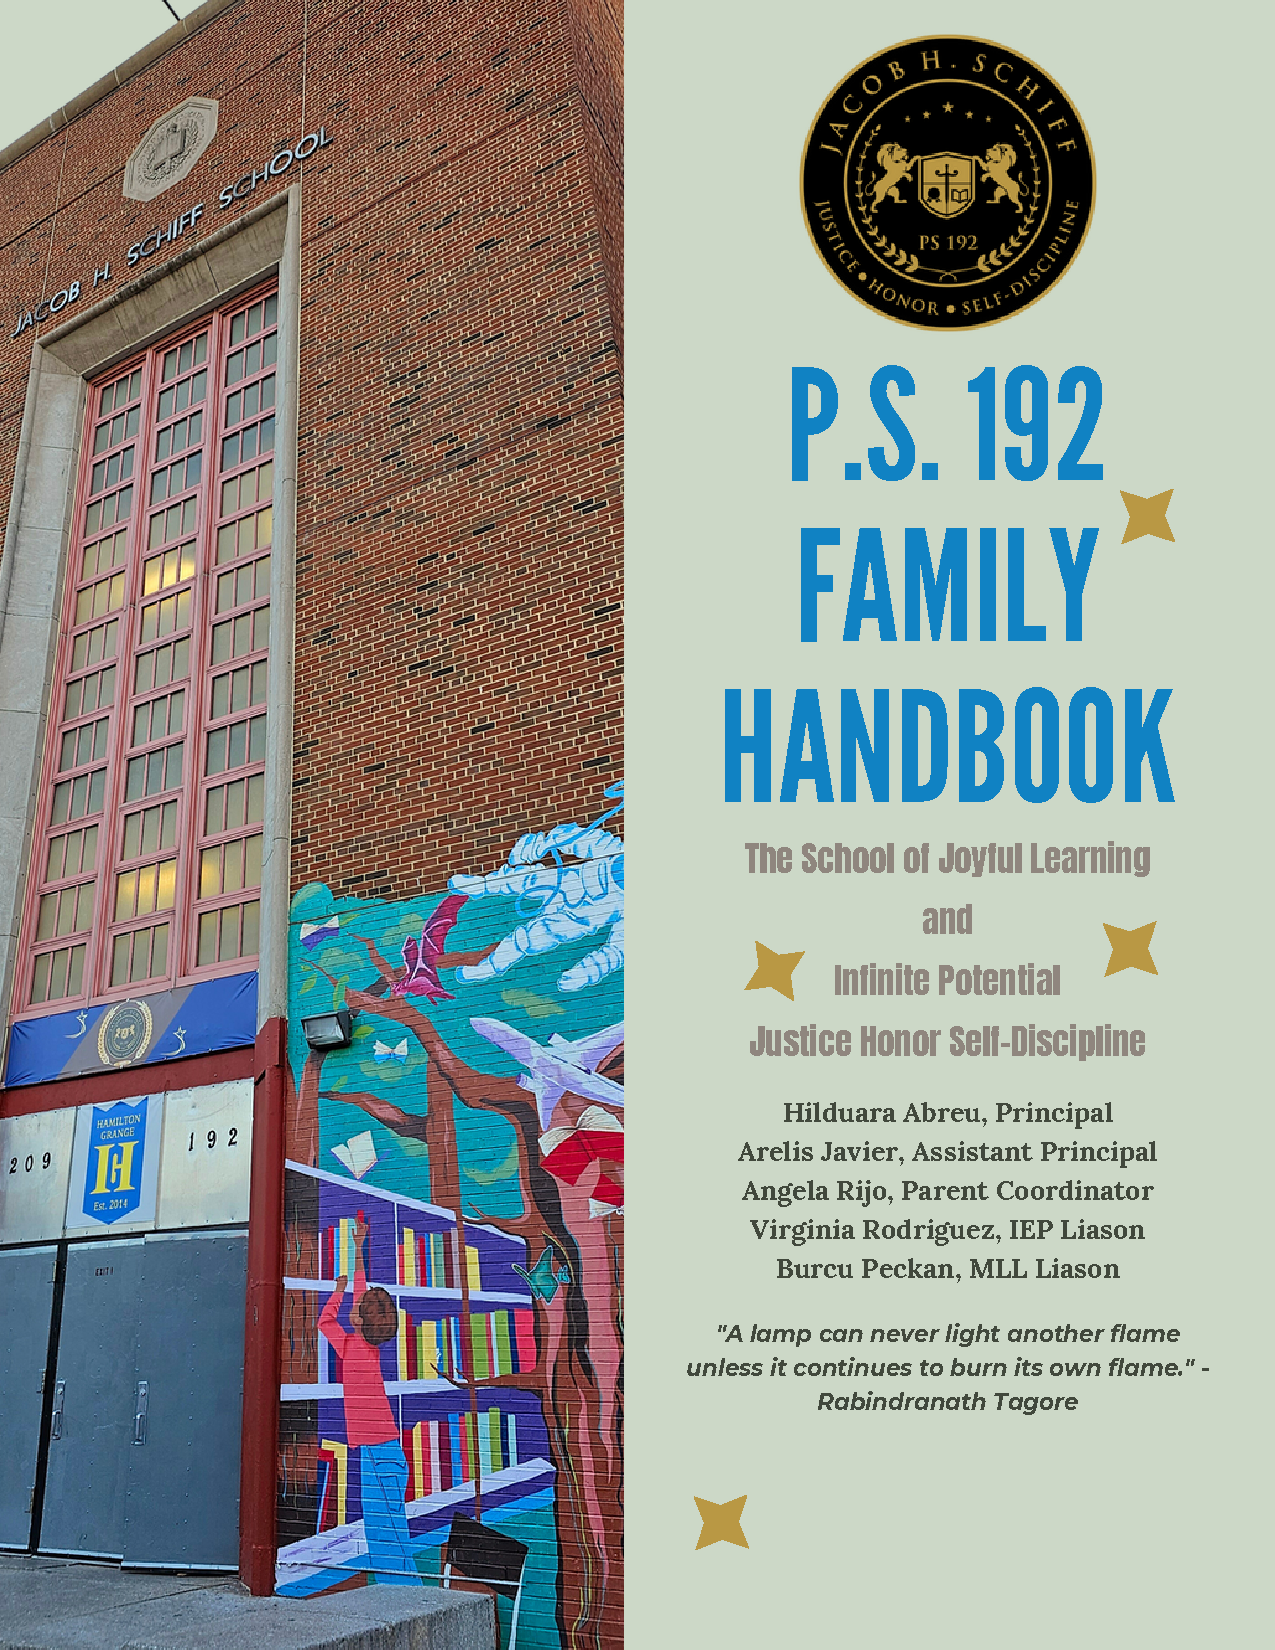
\includepdf[pages=1,fitpaper]{pdf.pdf}

\pagenumbering{\fancyhf{}}
\pagestyle{headings}
\pagenumbering{arabic}

\fancyhead[R]{\thepage}

\fancyfoot[C]{The School of joyful Learning \& Infinite Potential}
\pagestyle{fancy}
\renewcommand{\footrulewidth}{1px}

\definecolor{dkgreen}{rgb}{0,0.6,0}
\definecolor{gray}{rgb}{0.5,0.5,0.5}
\definecolor{mauve}{rgb}{0.58,0,0.82}

\clearpage
\clearpage \tableofcontents \clearpage
\section{Introduction}
\label{sec:org110a480}
This handbook serves as a guide to the policies, procedures, and expectations at PS 192 for the 2023-2024 school year. Please note that this document is subject to change throughout the year in response to New York City Department of Education (NYC DOE) updates, evolving needs within our school community, or other circumstances that may arise. This is a living document designed for the PS 192 school community, and we will keep families informed of any significant updates.

\section{Welcome!}
\label{sec:org6a4cc3f}
Dear Families,

Welcome to PS 192 for the 2024-2025 school year. At PS 192, we are proud of our commitment to joyful learning, where every child is encouraged to explore, discover, and grow in a supportive environment. We look forward to working with you and your child to provide every opportunity for success. We invite you to be active participants in our school community.

With Justice, Honor, and Self-discipline,

Ms. Hilduara Abreu, Principal
Dr. Milagros Dueno, Assistant Principal
Ms. Arelis Javier, Assistant Principal
Ms. Angela Rijo, Parent Coordinator
Ms. Dulce Infante, School Secretary

\section{About PS 192}
\label{sec:orgb861cdf}
PS 192 is a diverse elementary school located in Harlem, NYC. Our mission is to provide students with a rich and rigorous academic program while fostering a supportive community where every child feels safe and valued.

Our Core Values:
\begin{itemize}
\item \textbf{\textbf{Justice}}
\item \textbf{\textbf{Honor}}
\item \textbf{\textbf{Self-discipline}}
\end{itemize}

These values guide everything we do, from our classroom instruction to our school-wide initiatives.

\textbf{\textbf{School-Wide Norms}}:
\begin{itemize}
\item We take care of ourselves.
\item We take care of each other.
\item We take care of our community.
\end{itemize}

\section{Key Information for Families}
\label{sec:org3ff6ab0}
\subsection{Key Contacts}
\label{sec:org464e1dd}
Below are the key contacts for this school year:

\begin{itemize}
\item \textbf{\textbf{Principal}}: Ms. Hilduara Abreu (habreu@ps192.org)
\item \textbf{\textbf{Assistant Principals}}: Dr. Milagros Dueno, Ms. Arelis Javier
\item \textbf{\textbf{Parent Coordinator}}: Ms. Angela Rijo (arijo@ps192.org)
\item \textbf{\textbf{School Secretary}}: Ms. Dulce Infante
\item \textbf{\textbf{Main Office Phone}}: 212-XXX-XXXX
\end{itemize}

\subsection{School Day Schedule}
\label{sec:org77d92b9}
\begin{itemize}
\item School hours: 8:30 AM - 2:50 PM
\item Breakfast: 8:00 AM - 8:25 AM
\end{itemize}

Please ensure your child arrives on time each day. Punctuality is crucial to their learning experience.

\subsection{Arrival and Dismissal}
\label{sec:org0a938ce}
\begin{itemize}
\item \textbf{\textbf{Arrival}}: Students can enter the building at 8:15 AM. Those having breakfast may arrive as early as 8:00 AM.
\item \textbf{\textbf{Dismissal}}: Dismissal is at 2:50 PM. Please be prompt in picking up your child.
\end{itemize}

\subsection{Late Arrivals}
\label{sec:orgfec3b88}
If your child arrives after 8:30 AM, they must report to the main office for a late pass.

\subsection{Early Dismissal}
\label{sec:orgb534b81}
If you need to pick up your child early, please email us at \texttt{dismissal@ps192.org} before 11 AM, and arrive no later than 2:30 PM for early pickup.

\subsection{Attendance and Absences}
\label{sec:orgae5d8b5}
Regular attendance is critical to your child's success. If your child is absent, please email \texttt{attendance@ps192.org} each day they are absent. A doctor's note is required after two consecutive days of absence.

\subsection{Breakfast, Lunch, and Snacks}
\label{sec:orge11dba2}
PS 192 offers free breakfast and lunch to all students. We are committed to healthy eating, and snacks brought from home should be nutritious and nut-free.

\section{Wellness and Healthy Eating}
\label{sec:orgf252f78}
PS 192 encourages healthy habits, including proper nutrition and physical activity. Children should bring a water bottle to school and wear comfortable, weather-appropriate clothing for outdoor play.

\begin{itemize}
\item \textbf{\textbf{No Nut Policy}}: Due to allergies, PS 192 is a nut-free school.
\item \textbf{\textbf{No Junk Food Policy}}: Please avoid sending candy, chips, or sugary snacks. Gum is not allowed in school.
\end{itemize}

\section{Family Engagement}
\label{sec:org20620d2}
\subsection{Parent Involvement}
\label{sec:orgfeded68}
At PS 192, we believe in building strong partnerships with families. Parents and guardians are encouraged to volunteer and participate in school events.

\subsection{Class Parents}
\label{sec:org7d7c842}
Class parents help facilitate communication between teachers and parents, assist with organizing classroom events, and coordinate volunteer efforts. If you are interested in becoming a class parent, please speak with your child's teacher.

\subsection{Parents’ Association}
\label{sec:orgbcdc52f}
All parents are automatically members of the PS 192 Parents’ Association (PA). The PA works with the school to organize events, raise funds, and support the school's mission. Monthly PA meetings are held to discuss important topics and build community.

\section{Curriculum and Instruction}
\label{sec:org1573ebd}
PS 192 follows a comprehensive curriculum that integrates literacy, math, social studies, and science. We also focus on social-emotional learning, emphasizing respect, responsibility, and empathy.

\subsection{Looping}
\label{sec:orgefeaa5a}
At PS 192, we use the looping model where students stay with the same teacher for two years, ensuring continuity and deep relationships between teachers and students.

\subsection{Assessment and Student Progress}
\label{sec:org2e9802e}
We regularly assess student progress through a combination of formative and summative assessments. Report cards are distributed three times a year, and student-led conferences are held to discuss goals and progress.

\begin{itemize}
\item \textbf{\textbf{Standardized Testing}}: Students in grades 3-5 participate in NY State English Language Arts (ELA) and Mathematics exams, as well as the Science exam in 5th grade.
\end{itemize}

\section{Discipline Policies and Procedures}
\label{sec:org759be53}
PS 192 follows the NYC DOE Discipline Code. Our approach to discipline emphasizes restorative justice and logical consequences, ensuring students understand the impact of their behavior and are supported in making better choices.

\subsection{Cell Phones and Electronic Devices}
\label{sec:org9ab75f5}
Cell phones and electronic devices must be turned off and stored away during the school day. If a student needs to contact a parent, they must go to the main office.

\subsection{Logical Consequences}
\label{sec:org0e93269}
\begin{itemize}
\item \textbf{\textbf{Take a Break}}: A student may take a brief break to regain control if they are feeling overwhelmed.
\item \textbf{\textbf{Loss of Privileges}}: If a student misuses a material or behaves inappropriately, they may lose the privilege temporarily.
\item \textbf{\textbf{Restorative Justice}}: Students are encouraged to "fix" their mistakes, whether it’s through an apology or a community service activity.
\end{itemize}

\section{Communication}
\label{sec:org64baec1}
PS 192 uses several communication methods to keep families informed:
\begin{itemize}
\item \textbf{\textbf{School Website}}: Visit \texttt{www.ps192.org} for important updates and resources.
\item \textbf{\textbf{Emails}}: Weekly emails are sent out with information about upcoming events and school news.
\item \textbf{\textbf{Newsletters}}: Monthly newsletters provide detailed updates on classroom activities and school-wide initiatives.
\end{itemize}

\subsection{Parent-Teacher Communication}
\label{sec:org1e8a126}
Parents are encouraged to maintain open lines of communication with teachers. Teachers will share their preferred method of communication at the start of the year. If you have concerns, please contact your child’s teacher to schedule a meeting.

\section{Health and Safety}
\label{sec:org1cb1394}
\subsection{School Nurse}
\label{sec:org128b1e0}
PS 192 has a full-time school nurse to address any medical needs. Please ensure all emergency contact information is up to date.

\subsection{Medication}
\label{sec:orgc602d48}
If your child requires medication during school hours, please submit the appropriate 504 medical form to the nurse’s office.

\subsection{Illness}
\label{sec:org7ff59e2}
Children should stay home if they are feeling unwell. Please notify the school if your child contracts a communicable disease, so we can inform other families.

\subsection{Emergencies}
\label{sec:org33d39c7}
In the event of an emergency, PS 192 follows NYC DOE procedures. Parents will be notified immediately if necessary. It is essential to keep all contact information current with the school office.

\section{School Culture and Traditions}
\label{sec:org1203eca}
PS 192 has several beloved traditions that help foster a sense of community and school spirit. These include:

\begin{itemize}
\item \textbf{\textbf{Town Meetings}}: Weekly assemblies where students and staff come together to celebrate achievements and discuss school-wide topics.
\item \textbf{\textbf{Family Breakfasts}}: Held twice a year, families join their children in the classroom for a morning of food, activities, and performances.
\item \textbf{\textbf{Moving Up Ceremony}}: At the end of the year, we celebrate our students as they transition to the next grade.
\end{itemize}

\section{Appendix}
\label{sec:orgc3868b1}
\subsection{Attendance Policy}
\label{sec:org5750912}
Regular attendance is essential for academic success. Students must maintain a minimum attendance rate of 90\%. Absences due to illness or family emergencies must be communicated to the school office.

\subsection{Bussing and Transportation}
\label{sec:org4755b60}
PS 192 offers bussing for eligible students. Please contact the Parent Coordinator for more information about transportation options.

\subsection{Volunteer Guidelines}
\label{sec:orgd912ac4}
Parents are welcome to volunteer in classrooms, field trips, and school events. All volunteers must complete a background check and provide proof of vaccination.

\subsection{School Supplies}
\label{sec:org35e40d7}
PS 192 provides most school supplies. Students are asked to bring a backpack, water bottle, and any personal items as needed.
\end{document}
